

\section{Android app architecture}
The app runs on the users' Android device and was designed to run on Android version 4.0 or greater. As of March 2014 this makes up for 79,7\% of Android devices~\cite{AndroidDeviceFragmentation}. The team decided to only adapt the app for these versions because the app is a proof-of-concept, and for the purposes of the app, the team assumed that the relevant users would have a relatively modern phone. 

The architecture heavily relied on using ContentProviders~\cite{contentproviders} for database access. This gives the app a uniform access model for the data that does not run on the UI thread. When lists of data are accessed from an Activity or a Fragment, the LoaderManagers~\cite{loadermanager} is used. This handles the life cycle of data change notification through the cursor. 

The remaining problem was where to place the business logic for data manipulation. This is where the pattern Model-View-Presenter (MVP) comes in. MVP is a Model-View-Controller (MVC) derivative.~\cite{mvc} All business logic is handled in presenter classes. Through this uniform access, all logic applied to data preservation (sever synchronization), and data control can be handled in one place. The life cycle of the presenter classes is in the base Activity class, and all other sub fragments can get access to it though a interface. This pushes almost all logic into the presenters, making the code in the fragments as minimal as possible.

The app will follow standard Android design guidelines regarding the user interface design.

\todo{update architecture illustration to current solution}
\todo{class diagram front-end}
\todo{add figures if it help explaning}

\begin{figure}[H]
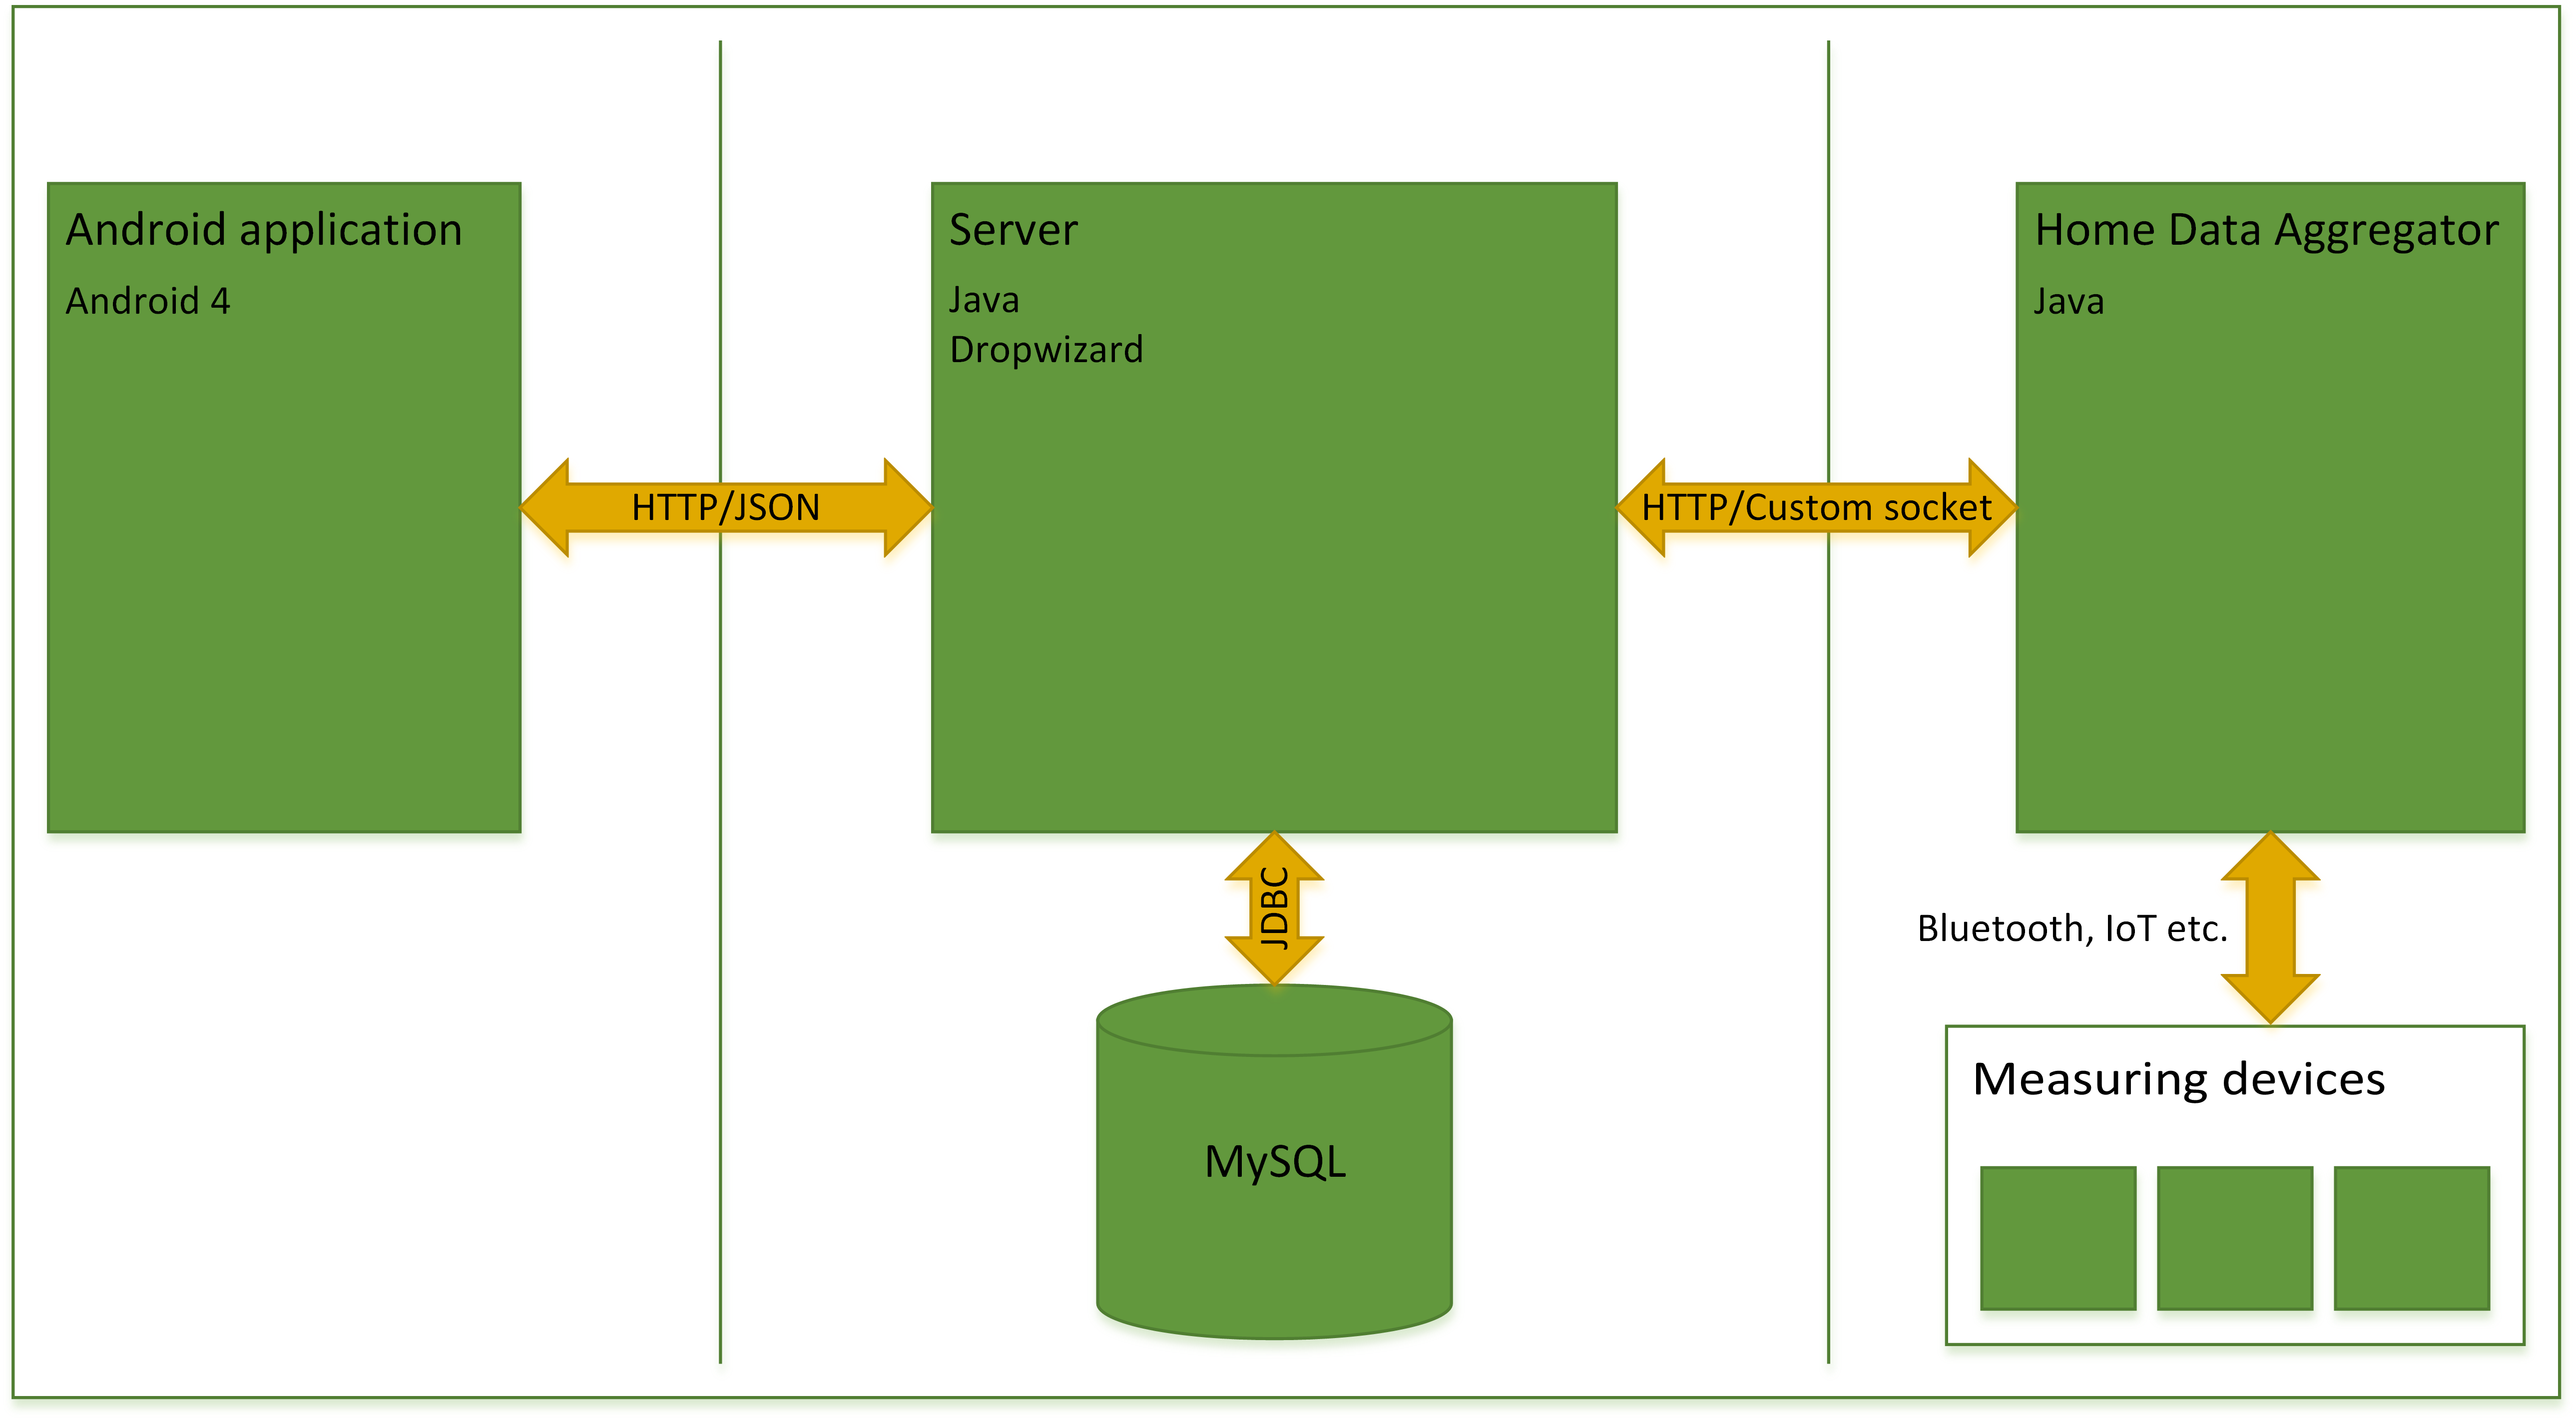
\includegraphics[width=\textwidth]{ch/architecture/fig/architecture.png}
\caption{Architecture overview}
\end{figure}

\subsection{Patterns}
\subsubsection{Model View Presenter}

\todo{Write about MVP and other patterns that we follow}